% PS_and_deltadef
\documentclass{standalone}

\usepackage{tikz}
    
\usepackage{graphicx} % Работа с графикой \includegraphics{}
\graphicspath{{./images/img1/}} % картинки в папке ./images/img1/
    
\begin{document}

\begin{tikzpicture}[x=10.0cm,y=10.0cm]
    \node[anchor=south west,inner sep=0] at (0,0) {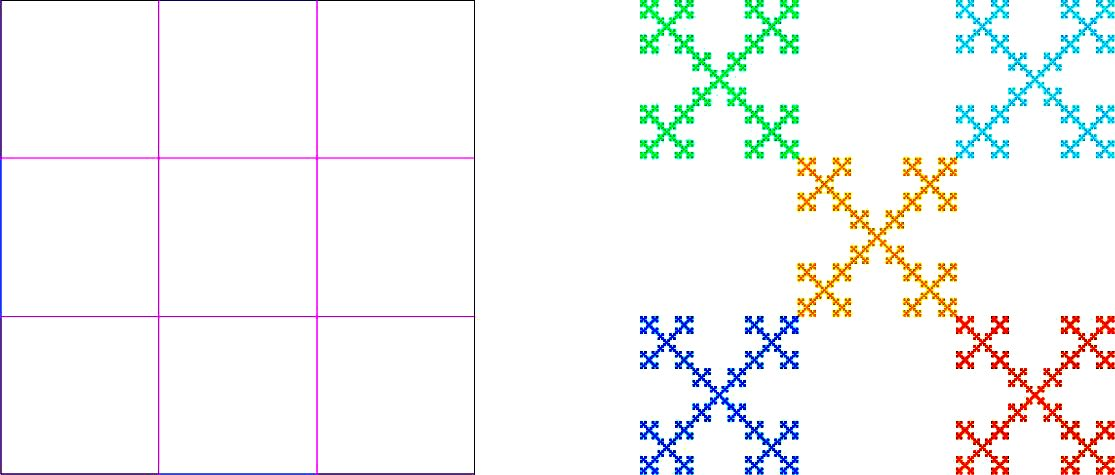
\includegraphics[width=7.31cm]{def0.jpg}};
    \node[anchor=south west,inner sep=0] at (0.855,0) {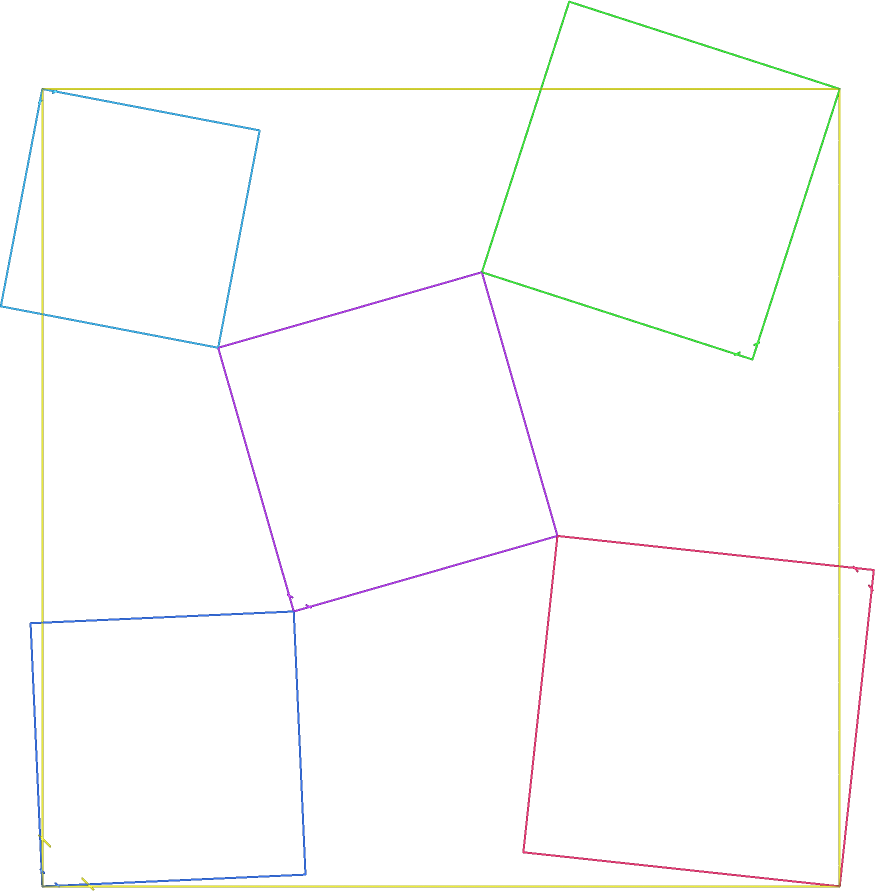
\includegraphics[width=3.5cm]{p1s.png}};
    \node[anchor=south west,inner sep=0] at (1.3,0) {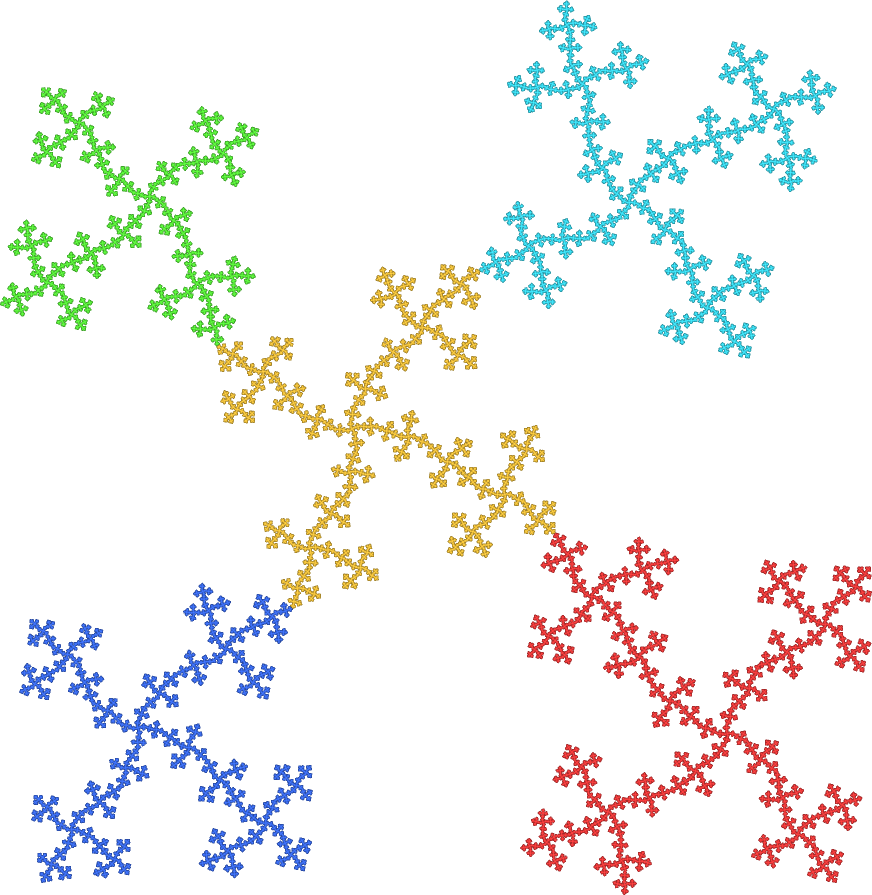
\includegraphics[width=3.5cm]{p1a.png}};
    %\draw[step=.01,yellow,very thin] (0,-.1) grid (1.7,.35);
    %\draw[step=.1,green,very thin] (0,-.1) grid (1.7,.35);
    \node at(0.27,.25){$P_3$};
    \node at (.15,.15) {$P_5$};
    \node at (.27,.05) {$P_2$};
    \node at (.05,.25) {$P_4$};
    \node at (0.05,.05) {$P_1$};
    \node at (1.12,.27){$P'_3$};
    \node at (1.0,.17) {$P'_5$};
    \node at (1.13,0.06) {$P'_2$};
    \node at (0.9,.27) {$P'_4$};
    \node at (.93,.06){$P'_1$};
\end{tikzpicture}

\end{document}